%%%% SI_Chapter4
%% Table S1

\begin{table}[h!]
\renewcommand{\baselinestretch}{1}
\renewcommand{\arraystretch}{1.2}
\begin{center}\fontsize{9}{11}\selectfont
\caption[Number of species for which RMR data was collected in each class \& data sources, initial RMR coverage for PREDICTS species and phylogenetic signal in RMR]{\textbf{Number of species for which RMR data was collected in each class \& data sources, initial RMR coverage for PREDICTS species and phylogenetic signal in RMR.}}
\label{SI5_table1}  
\begin{tabular}{|l|l|l|c|}
\hline
\textbf{Class}      & \multicolumn{1}{c|}{\textbf{RMR data}}                                                                                                         & \multicolumn{1}{c|}{\textbf{Coverage for PREDICTS species}} & \textbf{Phylogenetic signal (Pagel's $\lambda$, $\pm$95\% CI)} \\ \hline
\textbf{Amphibians} & \begin{tabular}[c]{@{}l@{}}126 species from\\ \citet{Stark2020}\end{tabular}                                                                 & 16/379 species (4\%)                                        & 0.89 (0.86-0.91)                              \\ \hline
\textbf{Birds}      & \begin{tabular}[c]{@{}l@{}}719 species from\\ \citet{McNab2009} \\ \citet{Fristoe2015} \\ \citet{Londono2015} \\ \citet{Stark2020} \end{tabular} & 317/3129 species (10\%)                                     & 0.97 (0.95-0.98)                              \\ \hline
\textbf{Mammals}    & \begin{tabular}[c]{@{}l@{}}685 species from \\ PanTHERIA \citep{Jones2009}\\ \citet{Fristoe2015}\\ \citet{Stark2020} \end{tabular}        & 148/556 species (27\%)                                      & 0.99 (0.98-0.99)                              \\ \hline
\textbf{Reptiles}   & 173 species from \citet{Stark2020} & 24/329 species (7.3\%)                                      & 0.90 (0.86-0.92)                              \\ \hline
\end{tabular}
\end{center}
\end{table}

\vspace{2cm}


\begin{figure}[h!]
\centering
\fbox{\begin{minipage}{35em}
\text{log(Abundance)} = \text{LU} + \text{LUI} + \text{TG} + \text{log(BM)} + \\
\text{LU}:\text{LUI} + \text{LU}:\text{TG} + \text{LU}:\text{log(BM)} +
\text{LUI}:\text{TG}  + \text{LUI}:\text{log(BM)} + \text{TG}:\text{log(BM)} + \\
  \text{LU}:\text{TG}:\text{log(BM)} + \text{LUI}:\text{TG}:\text{log(BM)} \
\end{minipage}}

\caption[Formula for the abundance model, used to understand the role of shifts in the body mass of species on observed changes in tRMR]{Formula for the abundance model, used to understand the role of shifts in the body mass of species on observed changes in tRMR (see main text, `Disentangling the effects of body mass and abundance on tRMR'). I fitted a model to explain changes in species abundance (given presence) by land use, land-use intensity, trophic group, body mass and their interactions. The model included all two-way interactions among these predictors. To account for potential differences in the slope of the relationship between abundance and body mass among the different trophic groups, I also included two three-way interactions in the model (among land use, trophic group and body mass; and among land-use intensity, trophic group and and body mass). Random effects included study, site and species identity. LU: land use; LUI: land-use intensity; TG: trophic group; BM: body mass.}
\label{SI5_figure1}
\end{figure}


%% Predictions for abundance model
\begin{figure}[h!]
\centering
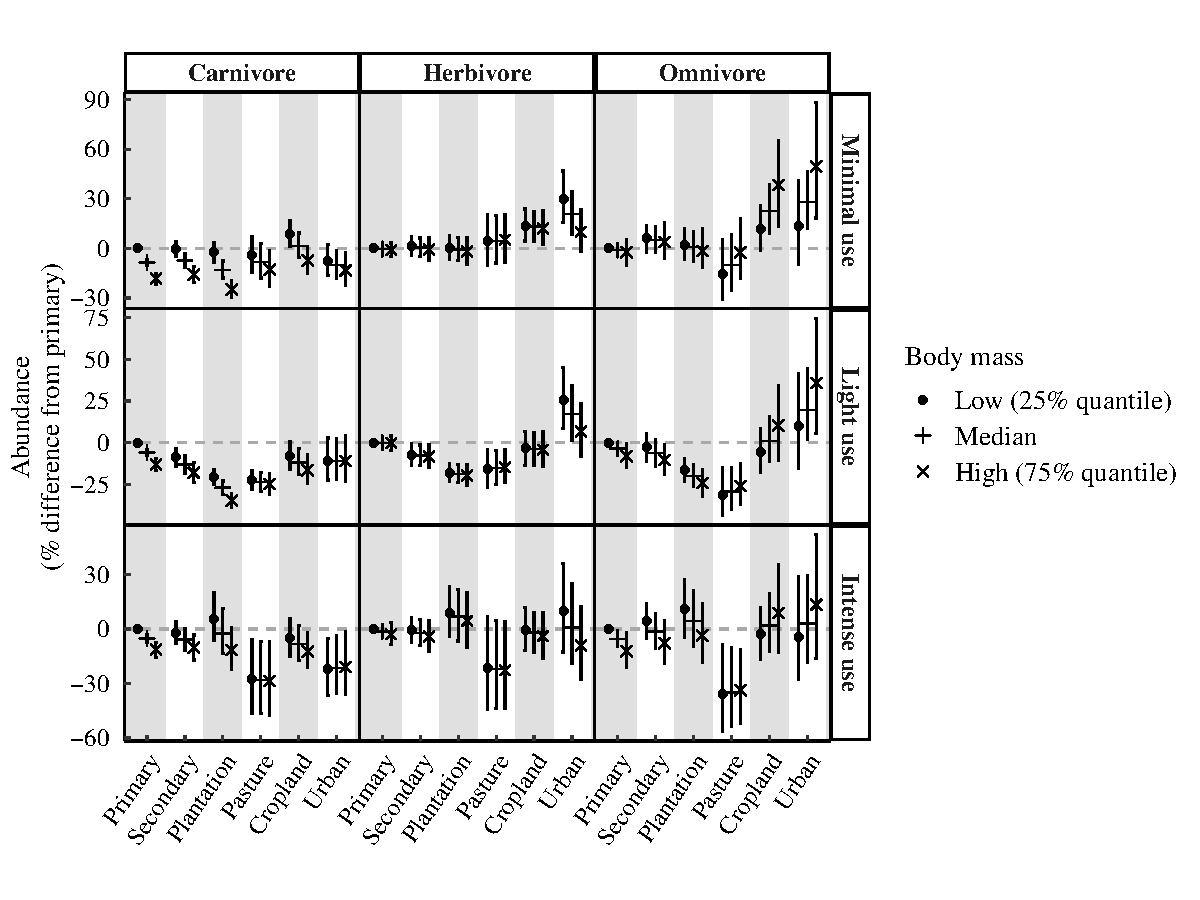
\includegraphics[scale=0.9]{Supporting/Chapter5/Figures/Figure_Abundance_difference}
\caption[Effects of land use, land-use intensity, trophic group, body mass and their interactions on assemblage-level total abundance]{\textbf{Effects of land use, land-use intensity, trophic group, body mass and their interactions on assemblage-level total abundance}, estimated from the model specified in Figure \ref{SI5_figure1}. The predictions are rescaled with reference to minimally used primary vegetation, considered to be the undisturbed baseline. Primary: primary vegetation; secondary: secondary vegetation; plantation: plantation forest. For visualisation purposes, I plotted the predictions for three body mass levels (but body mass was considered as a continuous variable in the model).}
\label{SI5_figure2}
\end{figure}



%% Model diagnostic for total RMR
\begin{figure}[h!]
\centering
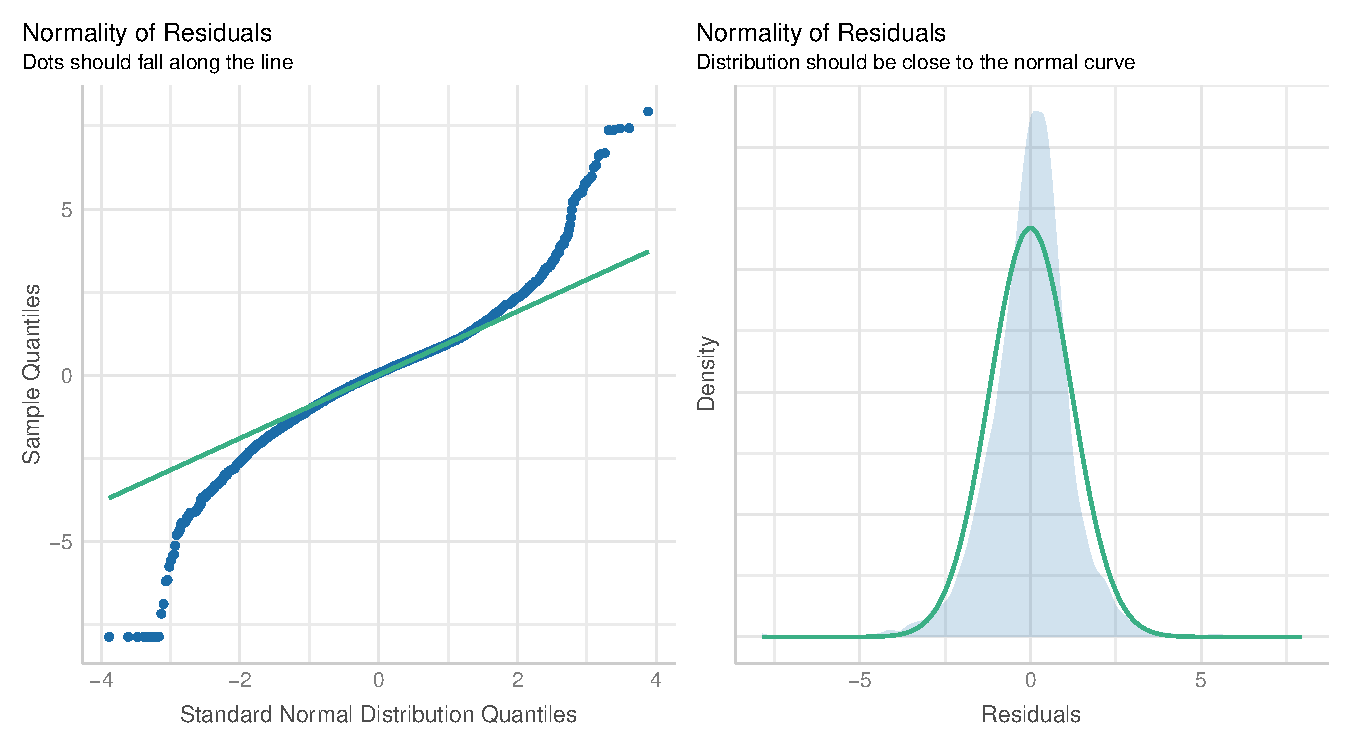
\includegraphics[scale=0.75]{Supporting/Chapter5/Figures/Diagnostics_tRMR}
\caption[Diagnostic plots for the linear mixed-effects model looking at the effects of land use, land-use intensity, trophic group and their interactions on assemblage-level total RMR]{\textbf{Diagnostic plots (qq-plot and residual distribution) for the linear mixed-effects model looking at the effects of land use, land-use intensity, trophic group and their interactions on assemblage-level total RMR.} The diagnostic plots were obtained with the `performance' R package \citep{performance}.}
\label{SI5_figure3}
\end{figure}

%% Model validation for total RMR: coefficients from the two models 
\begin{figure}[h!]
\centering
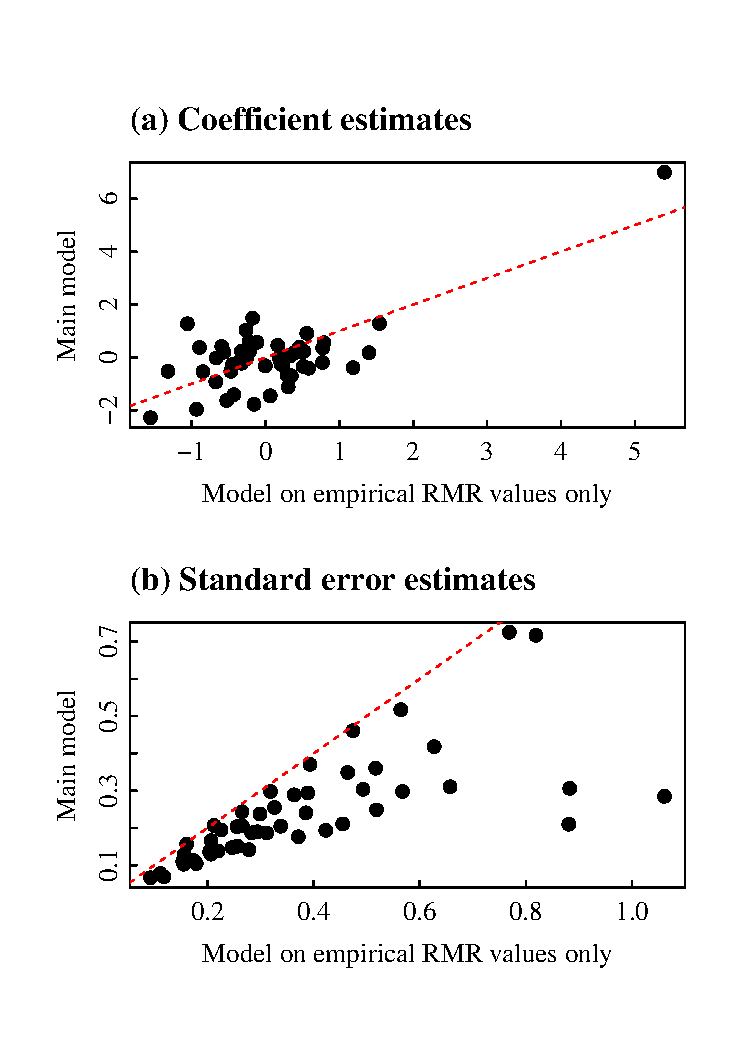
\includegraphics[scale=0.7]{Supporting/Chapter5/Figures/tRMR_coefs_complete_VS_imputed}
\caption[Estimates for the models looking at the effects of land use, land-use intensity, trophic group and their interactions on assemblage-level total RMR]{\textbf{Estimates for the models looking at the effects of land use, land-use intensity, trophic group and their interactions on assemblage-level total RMR.} I plotted the estimates from the model fitted on the empirical and imputed RMR values (presented in the main text) on the y-axis, and the estimates from the model fitted on the empirical RMR values only on the x-axis.}
\label{SI5_figure4}
\end{figure}


%% Model validation for total RMR: predictions from the two models
\begin{figure}[h!]
\centering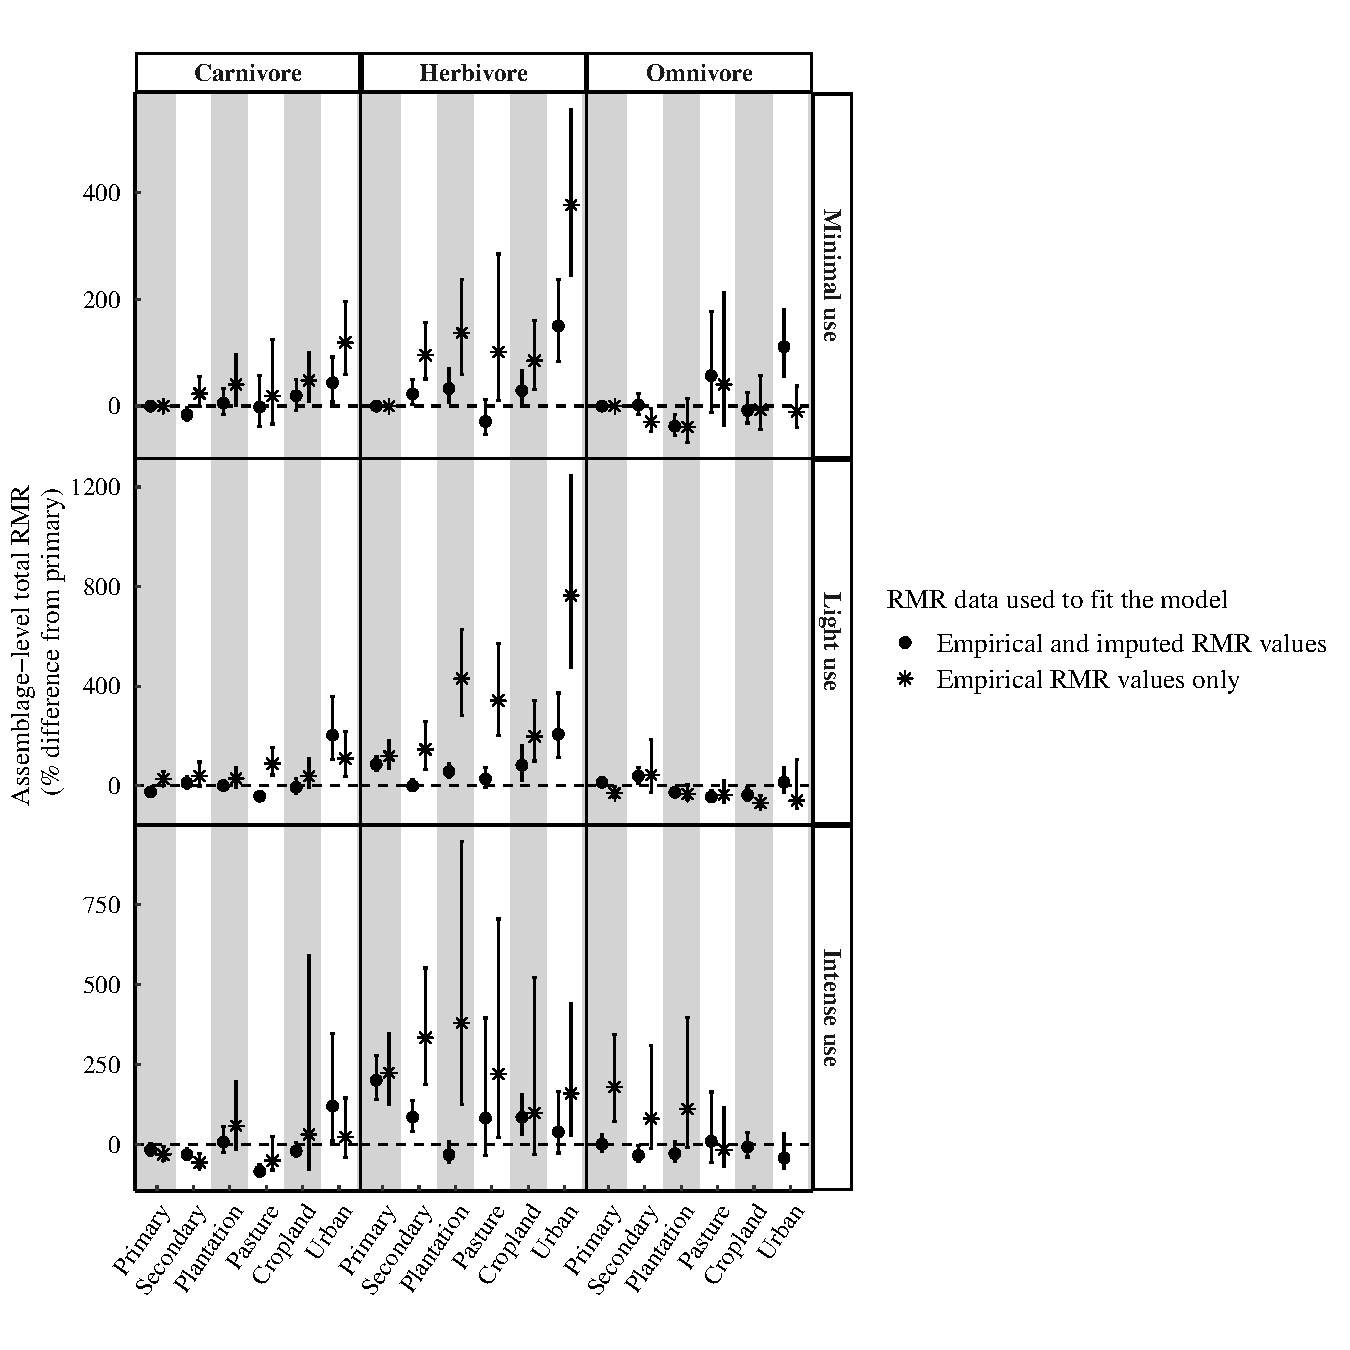
\includegraphics[scale=0.8]{Supporting/Chapter5/Figures/Complete_VS_imputed_total}
\caption[Effects of land use, land-use intensity, trophic level and their interactions on assemblage-level total RMR: empirical versus imputed]{\textbf{Effects of land use, land-use intensity, trophic level and their interactions on assemblage-level total RMR}, estimated from the model fitted on the empirical and imputed RMR values (presented in the main text) and from the model fitted on the empirical values only. The predictions are rescaled with reference to minimally used primary vegetation, considered to be the undisturbed baseline. Primary: primary vegetation; secondary: secondary vegetation; plantation: plantation forest.}
\label{SI5_figure5}
\end{figure}


%% Model diagnostics for occurrence model
\begin{figure}[h!]
\centering
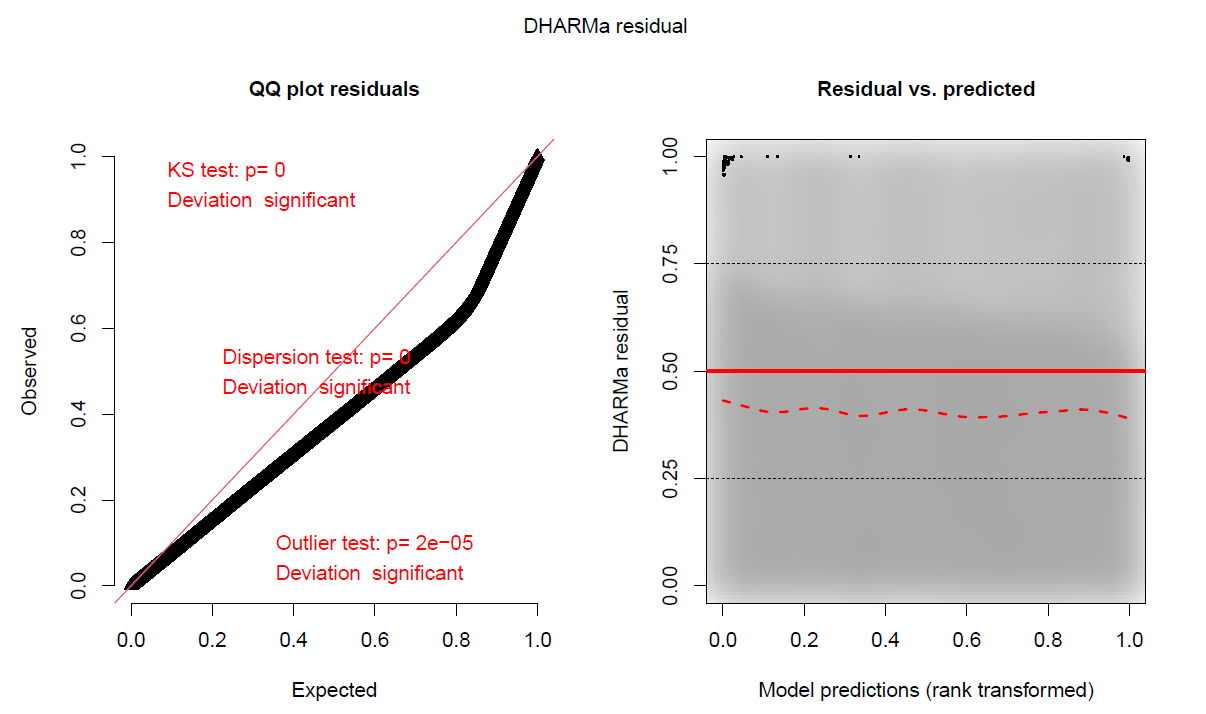
\includegraphics[scale=0.7]{Supporting/Chapter5/Figures/Diagnostic_plot_occurrence.png}
\caption[Diagnostic plots for the generalised mixed-effects model looking at the effects of land use, land-use intensity, trophic group, residual RMR and their interactions on species' probability of occurrence]{\textbf{Diagnostic plots for the generalised mixed-effects model looking at the effects of land use, land-use intensity, trophic group, residual RMR and their interactions on species' probability of occurrence.} The diagnostic plots were obtained with the `DHARMa' R package \citep{DHARMa}.}
\label{SI5_figure6}
\end{figure}

%% Bayesian model against Maximum likelihood
\begin{figure}[h!]
\centering
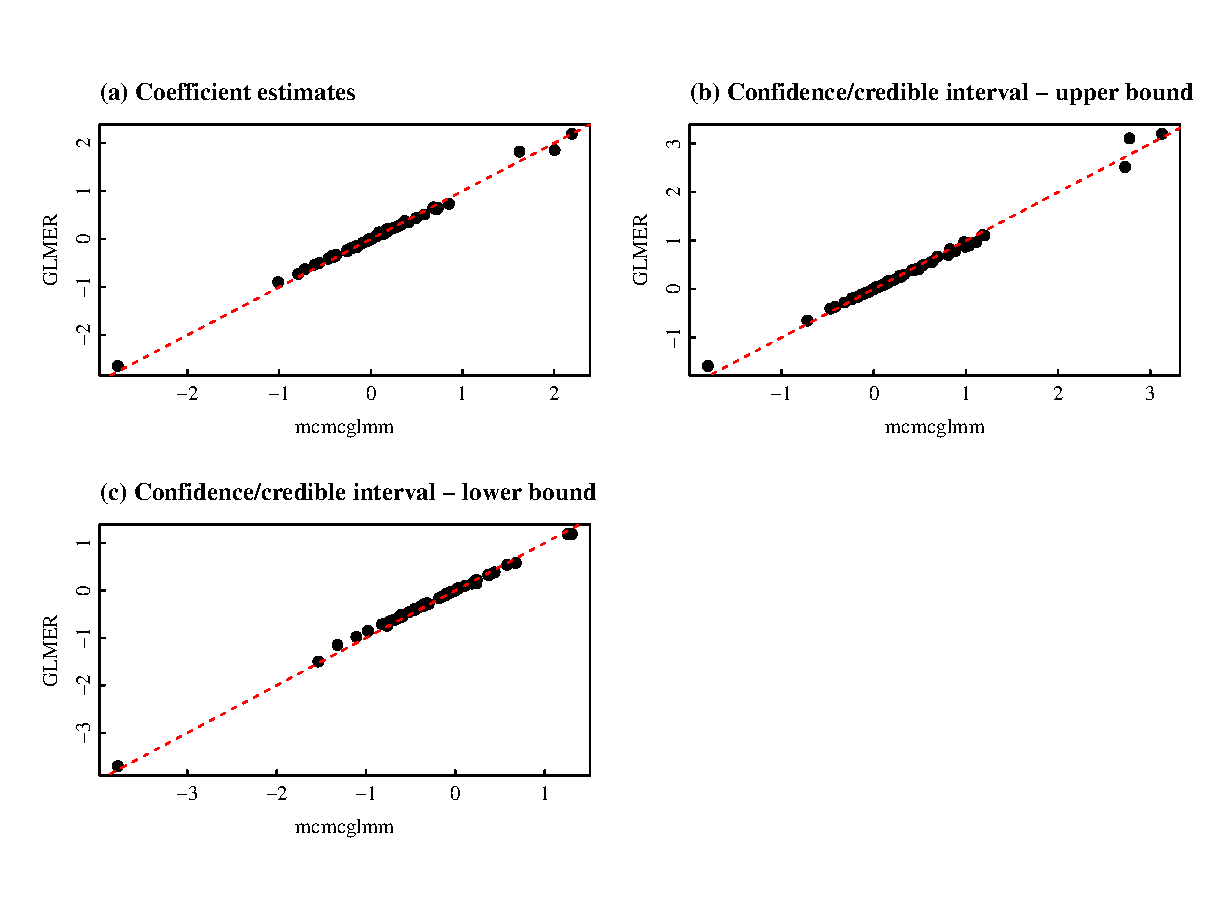
\includegraphics[scale=0.8]{Supporting/Chapter5/Figures/Occurrence_model_GLMER_mcmcglmm_coefs}
\caption[Model's coefficients from the occurrence model fitted using the `lme4' package against coefficients from the model fitted using the `MCMCglmm' package]{\textbf{Model's coefficients from the occurrence model fitted using the `lme4' package \citep{Bates2015} against coefficients from the model fitted using a Bayesian framework with the `MCMCglmm' package \citep{mcmcglmm}.} The models were fitted to investigate the effects of land use, land-use intensity, trophic group and residual RMR on species occurrence probability.}
\label{SI5_figure7}
\end{figure}

\newpage
%% Model validation for occurrence model
\begin{figure}[h!]
\centering
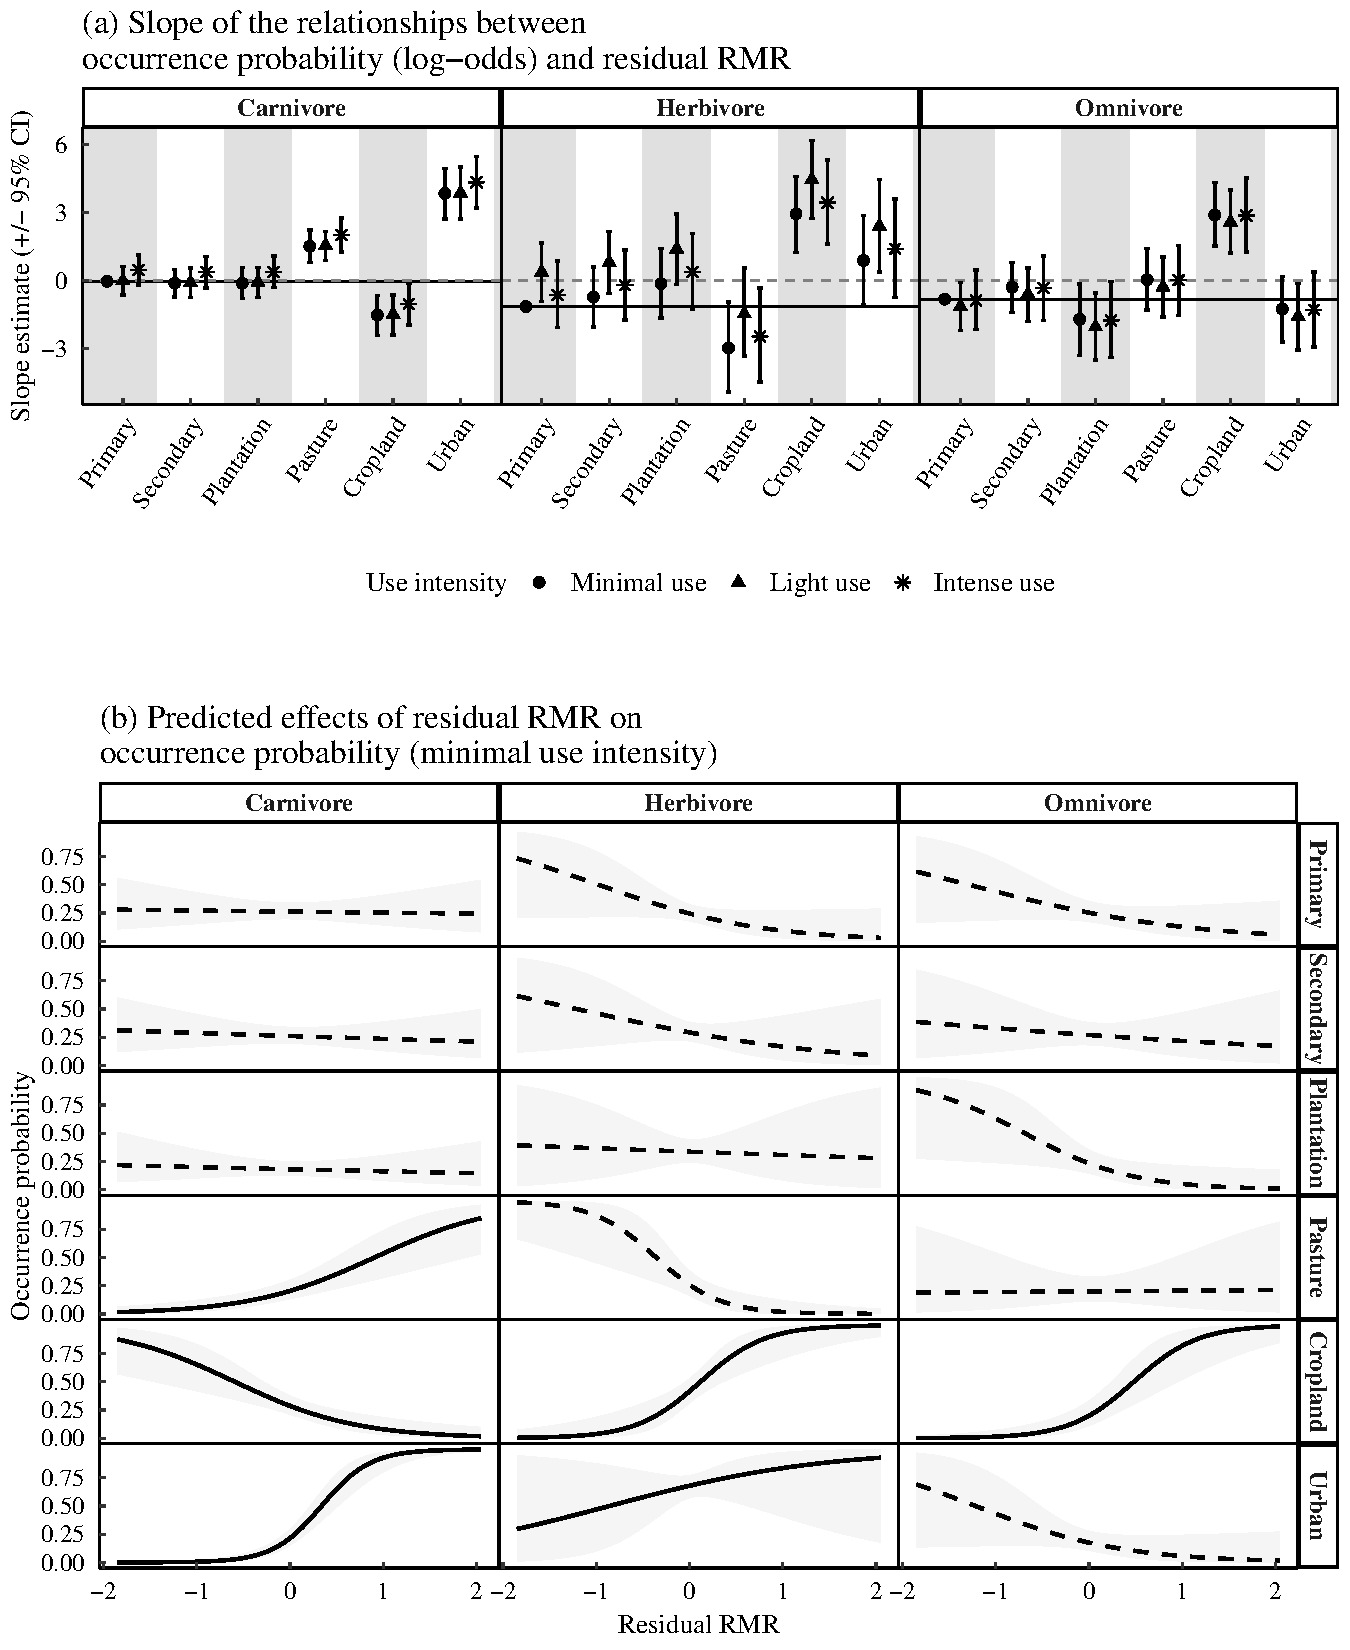
\includegraphics[scale=0.67]{Supporting/Chapter5/Figures/Figure_predictions_slopes_Complete_data_v2}
\caption[Slope estimates and predictions for the relationship between occurrence probability and residual RMR for the model fitted on empirical RMR values only]{\textbf{(a) Slope estimates for the relationship between residual RMR and occurrence probability in each land-use type and for the three levels of land-use intensity, from the model fitted using the empirical RMR values (i.e., excluding imputed RMR values).} The black horizontal line indicates the slope for the reference level (primary vegetation) for minimal land-use intensity. The grey dashed line marks 0. Error bars are 95\% confidence intervals. \textbf{(b) Effect of residual RMR on species probability of occurrence within each trophic level and for each land use-type.} I plotted the predictions for minimal land-use intensity only. Solid lines represent significant relationships. Primary: primary vegetation; secondary: secondary vegetation; plantation: plantation forest.}
\label{SI5_figure8}
\end{figure}

\clearpage